% Part: sets-functions-relations
% Chapter: relations
% Section: trees

\documentclass[../../../include/open-logic-section]{subfiles}

\begin{document}

\olfileid{sfr}{rel}{tre}
\olsection{বৃক্ষ}

একটি বিশেষ ধরনের আংশিক ক্রম, যা যুক্তিবিদ্যার সব শাখায় গুরুত্বপূর্ণ ভূমিকা পালন করে, হল \emph{বৃক্ষ}। যুক্তিবিদ্যার প্রাথমিক অংশে সসীম বৃক্ষ দেখা যায়: যেমন, !!{formula}sকে তাদের গঠন অনুসারে একটি বাক্যতাত্ত্বিক বৃক্ষে ভেঙে বোঝা যায়, আবার বহু !!{derivation} পদ্ধতিতে !!{derivation}sও সসীম বৃক্ষের আকার নেয়।
%
বচনমূলক এবং প্রথম-ক্রমের যুক্তিবিদ্যার পূর্ণতা উপপাদ্যের প্রমাণেই অসীম বৃক্ষের ব্যবহার দেখা যায়, এবং গাণিতিক যুক্তিবিদ্যার সর্বত্র এগুলি ব্যবহৃত হয়।

বৃক্ষের সেটতাত্ত্বিক ধারণাটি গ্রাফতত্ত্বের বৃক্ষ ধারণার ঘনিষ্ঠ। এখানে একটি (সসীম) বৃক্ষের ছবি দেওয়া হল:

\begin{center}
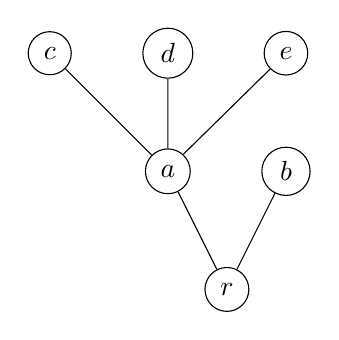
\begin{tikzpicture}[nodes={draw, circle}, -]
\node{$r$} [grow'=up]
    child { node {$a$}
        child { node {$c$} }
        child { node {$d$} }
        child { node {$e$} }
    }
    child { node {$b$} };
\end{tikzpicture}
\end{center}

সবচেয়ে নীচের নোড~$r$ হল মূল। $r$ ছাড়া প্রত্যেক নোডের ঠিক নীচে একটি মাত্র জনক নোড আছে। নোড~$x$ এবং নোড~$y$-এর মধ্যে এই সম্পর্কটি বিবেচনা করো: প্রান্ত বরাবর উপরের দিকে গিয়ে $x$ থেকে $y$-তে পৌঁছানো যায়। এই সম্পর্ককে $x$-এর $y$-এর \emph{পূর্বপুরুষ} হওয়া হিসেবে ভাবতে পারি।

বৃক্ষের পূর্বপুরুষ সম্পর্ক একটি কঠোর আংশিক ক্রম। এখান থেকেই সেটতাত্ত্বিক সংজ্ঞার প্রেরণা আসে। সংজ্ঞাটি দিতে আমাদের দুটি ধারণা দরকার। $\le$ দ্বারা আংশিকভাবে ক্রমিত সেট~$A$-এর একটি \emph{ক্ষুদ্রতম উপাদান} হল এমন !!a{element} $x \in A$, যার জন্য সকল $y \in A$-এর ক্ষেত্রে~$x \le y$ হয়। একটি সেট $\le$ দ্বারা \emph{সুক্রমিত} যদি তার প্রত্যেক অশূন্য উপসেটের ক্ষুদ্রতম উপাদান থাকে।

\begin{defn}[বৃক্ষ]
একটি \emph{বৃক্ষ} হল যুগল $T = \tuple{A, \le}$, যেখানে $A$ একটি সেট এবং $\le$, $A$-এর উপর আংশিক ক্রম; এর একটি অনন্য ক্ষুদ্রতম উপাদান $r \in A$ আছে (যাকে \emph{মূল} বলা হয়), এবং সকল $x \in A$-এর জন্য $\Setabs{y}{y \le x}$ সেটটি $\le$ দ্বারা সুক্রমিত।
\end{defn}

\begin{defn}[উত্তরসূরি]
ধরা যাক, $T = \tuple{A, \le}$ একটি বৃক্ষ। যদি $x,y \in A$, $x < y$, এবং এমন কোনো $z \in A$ না থাকে যাতে $x < z < y$ হয়, তবে আমরা $y$-কে $x$-এর \emph{উত্তরসূরি} বলি।
\end{defn}

$x \in A$-এর উত্তরসূরিদের তার \emph{সন্তান}ও বলা হয়। যদি $y$, $x$-এর উত্তরসূরি হয়, তবে $x$-কে $y$-এর \emph{পূর্বসূরি} বা \emph{জনক} বলি।

\begin{prop}
যদি $\tuple{A,\le}$ একটি বৃক্ষ হয়, তবে মূল ছাড়া প্রত্যেক $x \in A$-এর সর্বাধিক একজন পূর্বসূরি থাকে।
\end{prop}

\begin{proof}
  ধরা যাক $y_1 < x$ এবং $y_2 < x$ এবং $y_1 \neq y_2$। তাহলে $\{y_1, y_2\} \subseteq \Setabs{z}{z<x}$। যেহেতু $\Setabs{z}{z<x}$, $\le$ দ্বারা সুক্রমিত, তাই তার উপসেট $\{y_1, y_2\}$-এর ক্ষুদ্রতম উপাদান আছে, যা অবশ্যই হয় $y_1$, নয়তো~$y_2$। তাই হয় $y_1 \le y_2$, নয়তো $y_2 \le y_1$। আমরা $y_1 \neq y_2$ ধরে নিয়েছিলাম; তাই আসলে হয় $y_1 < y_2$, নয়তো $y_2 < y_1$। আবার যেহেতু আমরা $y_1 < x$ এবং $y_2 < x$ ধরে নিয়েছিলাম, তাই আরও পাই, হয় $y_1 < y_2 < x$, নয়তো $y_2 < y_1 < x$। সুতরাং $y_1$ ও $y_2$ উভয়েই $x$-এর পূর্বসূরি হতে পারে না।
\end{proof}

\begin{defn}
একটি বৃক্ষ $T = \tuple{A, \le}$-কে \emph{অসীম} বলা হয় যদি $A$ অসীম সেট হয়; অন্যথায় তাকে \emph{সসীম} বলা হয়। যদি $T$-তে প্রত্যেক $x \in A$-এর কেবল সসীমসংখ্যক উত্তরসূরি থাকে, তবে আমরা $T$-কে \emph{সসীম শাখায়িত} বলি।
\end{defn}

\begin{defn}[শাখা]
একটি বৃক্ষ $T = \tuple{A, \le}$ দেওয়া থাকলে, $T$-এর একটি \emph{শাখা} হল $T$-এর একটি অন্তর্ভুক্তির বিচারে সর্বাধিক শৃঙ্খল; অর্থাৎ এমন সেট $B \subseteq A$ যাতে যেকোনো $x, y \in B$-এর জন্য হয় $x \le y$, নয়তো $y \le x$, এবং যেকোনো $z \in X \setminus B$-এর জন্য এমন $u \in B$ আছে যাতে $z \le u$ বা $u \le z$ কোনোটিই হয় না।
%
$T$-এর সব শাখার সেট বোঝাতে আমরা $[T]$ ব্যবহার করি।
\end{defn}

\begin{ex}
সসীম শাখায়িত বৃক্ষের একটি পরিচিত উদাহরণ হল $0$ ও~$1$-এর সসীম অনুক্রমগুলি নিয়ে গঠিত \emph{অসীম দ্বিমিক বৃক্ষ}, যাকে কখনো কখনো $\{0,1\}^*$ বা~$\Bin^*$ দিয়ে বোঝানো হয় এবং প্রসারণ সম্পর্ক $\sqsubseteq$ দ্বারা ক্রমিত করা হয় (যেমন, $101 \sqsubseteq 101101$)। যেহেতু যেকোনো দ্বিমিক প্রতীকক্রমের শেষে একটি $0$ বা একটি $1$ যোগ করে তাকে সর্বদা বাড়ানো যায়, তাই এই বৃক্ষে অসীমসংখ্যক উপাদান আছে: প্রত্যেক উপাদান~$s$-এর ঠিক দুটি উত্তরসূরি আছে, $s0$ এবং~$s1$। এর মূল হল শূন্য অনুক্রম $\emptyseq$।
\end{ex}

\begin{ex}
আরও একটু সাধারণভাবে, স্বাভাবিক সংখ্যার সসীম অনুক্রমের সেট~$\Nat^*$-ও প্রসারণ সম্পর্ক~$\sqsubseteq$ সমেত একটি বৃক্ষ। এটি যে সসীম শাখায়িত নয় তা স্পষ্ট: প্রত্যেক $s \in \Nat^*$-এর অসীমসংখ্যক উত্তরসূরি~$sn$ আছে, প্রত্যেক $n \in \Nat$-এর জন্য একটি করে। $\sqsubseteq$-এর অধীনে বদ্ধ প্রত্যেক $A \subseteq \Nat^*$ হল $\Nat^*$-এর একটি \emph{উপবৃক্ষ}। (অর্থাৎ $A$ এমন যে $s \in A$ এবং $s' \sqsubseteq s$ হলে $s' \in A$-ও হয়।) সব সসীম বৃক্ষকে $\Nat^*$-এর সসীম উপবৃক্ষ হিসেবে প্রকাশ করা যায়।
\end{ex}

\begin{prop}[ক্যোনিগের সহায়ক উপপাদ্য]
যদি $T = \tuple{A,\le}$ একটি সসীম শাখায়িত অসীম বৃক্ষ হয়, তবে $T$-এর একটি অসীম শাখা আছে।
\end{prop}

গণনাযোগ্যতা তত্ত্বে বহুল ব্যবহৃত ক্যোনিগের সহায়ক উপপাদ্যের একটি বিশেষ ক্ষেত্র, যাকে \emph{দুর্বল ক্যোনিগের সহায়ক উপপাদ্য} বলা হয়, হল: $\{0,1\}^*$-এর যেকোনো অসীম উপবৃক্ষের একটি অসীম শাখা আছে।

\end{document}
